\chapter{CNN Inspection Pipeline}
\label{ch:cnn-pipeline}

\section{Choice of CNNs}
\label{sec:cnn-choice}

We use convolutional neural networks because prior work has shown that bitstream-derived representations contain learnable structure. Rettkowski et al. studied neural-network-based inspection of partial FPGA bitstreams. Chaudhuri and Chakrabarty used CNN-based learning to detect malicious FPGA bitstreams. Elnaggar et al. also used CNNs as part of a malicious-circuit detection pipeline. These results support the idea that bitstreams can be treated as structured data for classification, even without full bitstream reverse engineering~\cite{rettkowski2019partialbitstreams,chaudhuri2022cnnbitstreams,elnaggar2023learning}.

This project follows the same direction, but with a different systems goal. The model is not only trained for software accuracy. It must also be small enough and regular enough to synthesize into FPGA logic. CNNs are a good fit for this because they can operate on fixed-size image-like tensors and can be converted to hardware using tools such as hls4ml.

The classifier receives the preprocessed bitstream tensor from Chapter~\ref{ch:dataset-preprocessing}. The output is a binary prediction. The positive class is the RO-based malicious class. The negative class is the benign Coyote application class.

\section{Model Input and Classification Task}
\label{sec:model-input-task}

Each partial bitstream is converted into a grayscale image-like tensor through deterministic resizing. The tensor does not represent a natural image. It is a fixed-size layout of byte values sampled from the bitstream. This gives the CNN local neighborhoods of byte values from which it can learn statistical and spatial patterns.

The main classification task is binary:
\[
    y =
    \begin{cases}
        0, & \text{benign Coyote partial bitstream},\\
        1, & \text{RO-based malicious partial bitstream}.
    \end{cases}
\]

The main metrics are accuracy, F1, true positive rate, false positive rate, false negative rate, and ROC AUC. False negatives are especially important because they correspond to malicious bitstreams that would be accepted by the checker.

\section{Design Space}
\label{sec:cnn-design-space}

The CNN design space is explored in stages. The goal is to preserve useful detection quality while keeping the final hardware design practical. We therefore vary the model only along dimensions that affect both classification and hardware cost.

\begin{table}[t]
    \centering
    \caption{CNN design-space dimensions.}
    \label{tab:cnn-design-space}
    \begin{tabular}{p{0.24\linewidth} p{0.38\linewidth} p{0.26\linewidth}}
        \toprule
        \textbf{Dimension} & \textbf{Question} & \textbf{Main metrics} \\
        \midrule
        Input resolution &
        How much bitstream detail is retained &
        F1, FNR, ROC AUC \\
        \midrule
        CNN depth &
        How much model capacity is needed &
        F1, TPR, FPR \\
        \midrule
        Quantization &
        How little precision is enough &
        AUC, hls4ml parity, resources \\
        \midrule
        Pruning &
        How much sparsity can be introduced &
        AUC, sparsity, synthesis impact \\
        \bottomrule
    \end{tabular}
\end{table}

The main software sweep varies input resolution and depth. The tested resolutions include smaller inputs such as $128^2$ and larger inputs such as $256^2$ and $512^2$. Higher resolutions preserve more bitstream detail, but they also increase the cost of the synthesized checker. The depth sweep evaluates whether additional convolutional layers improve detection enough to justify the hardware cost.

\section{Software Detection Results}
\label{sec:software-detection-results}

Figure~\ref{fig:f1-resolution-depth} shows the main software result. F1 improves as input resolution and model depth increase. Small inputs lose information during resizing. Larger inputs preserve more byte-level structure and give the CNN more useful signal. Deeper models also improve classification up to the evaluated range.

\begin{figure}[t]
    \centering
    % Replace with the exported F1 heatmap from the presentation.
    % Recommended file name: figures/f1_resolution_depth.pdf
    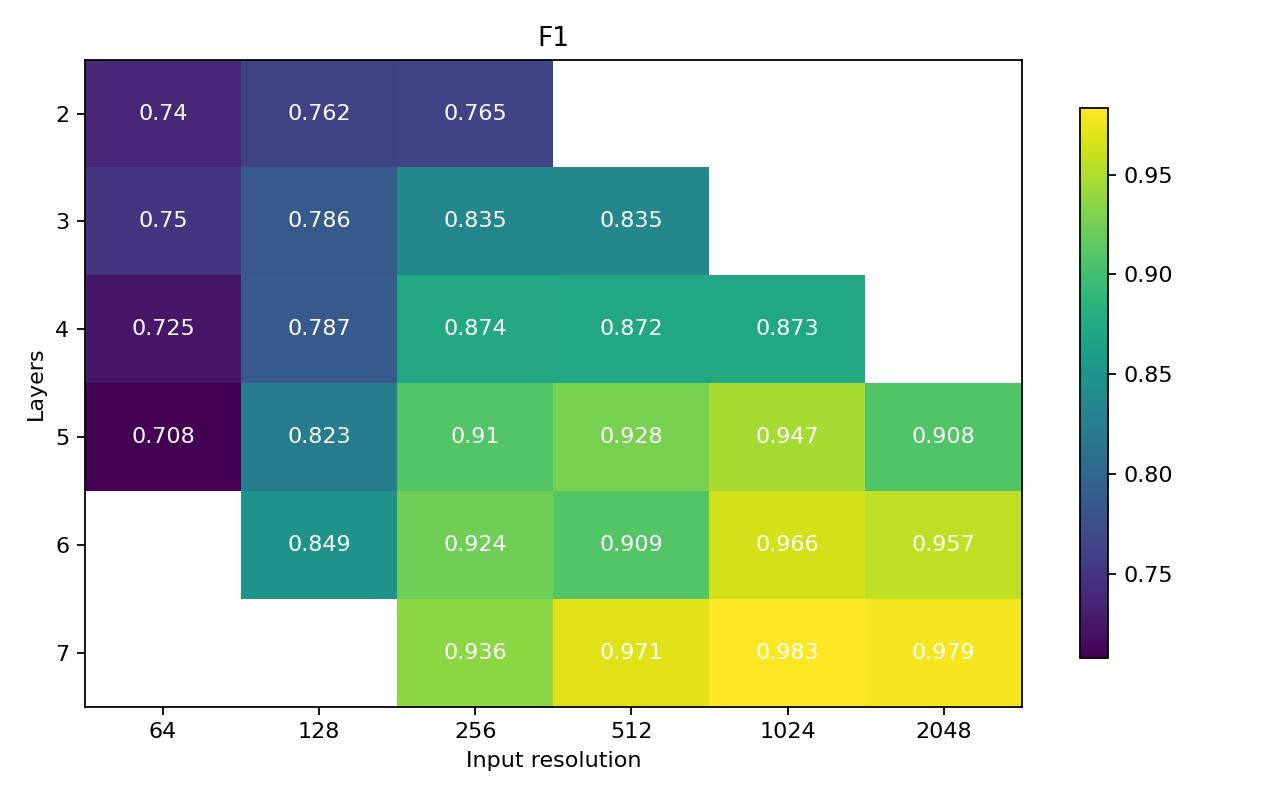
\includegraphics[width=0.82\linewidth]{figures/f1_resolution_depth.pdf}
    \caption{F1 score across input resolution and CNN depth. Higher resolution and deeper models improve software detection quality, but they also increase hardware cost.}
    \label{fig:f1-resolution-depth}
\end{figure}

The strongest software models are not automatically the best deployment candidates. Larger inputs improve F1, but they also increase memory pressure, latency, and resource usage after synthesis. The later hardware evaluation therefore focuses on deployable candidates rather than only the maximum-F1 software model.

\begin{table}[t]
    \centering
    \caption{Representative software CNN results.}
    \label{tab:software-cnn-results}
    \begin{tabular}{l r r r r}
        \toprule
        \textbf{Model} & \textbf{Resolution} & \textbf{Depth} & \textbf{F1} & \textbf{Role} \\
        \midrule
        256$\times$7 & $256^2$ & 7 & TODO & Deployment candidate \\
        512$\times$7 & $512^2$ & 7 & TODO & Accuracy-oriented candidate \\
        1024$\times$7 & $1024^2$ & 7 & TODO & Software upper-bound candidate \\
        \bottomrule
    \end{tabular}
\end{table}

\section{Interpretability Check}
\label{sec-interpretability}

We use Grad-CAM as a qualitative sanity check. The goal is to inspect whether the CNN focuses on localized regions of the bitstream image or behaves as if it only learned a trivial global statistic.

\begin{figure}[t]
    \centering
    % Optional. Replace with the Grad-CAM figure from the presentation.
    % Recommended file name: figures/gradcam_example.pdf
    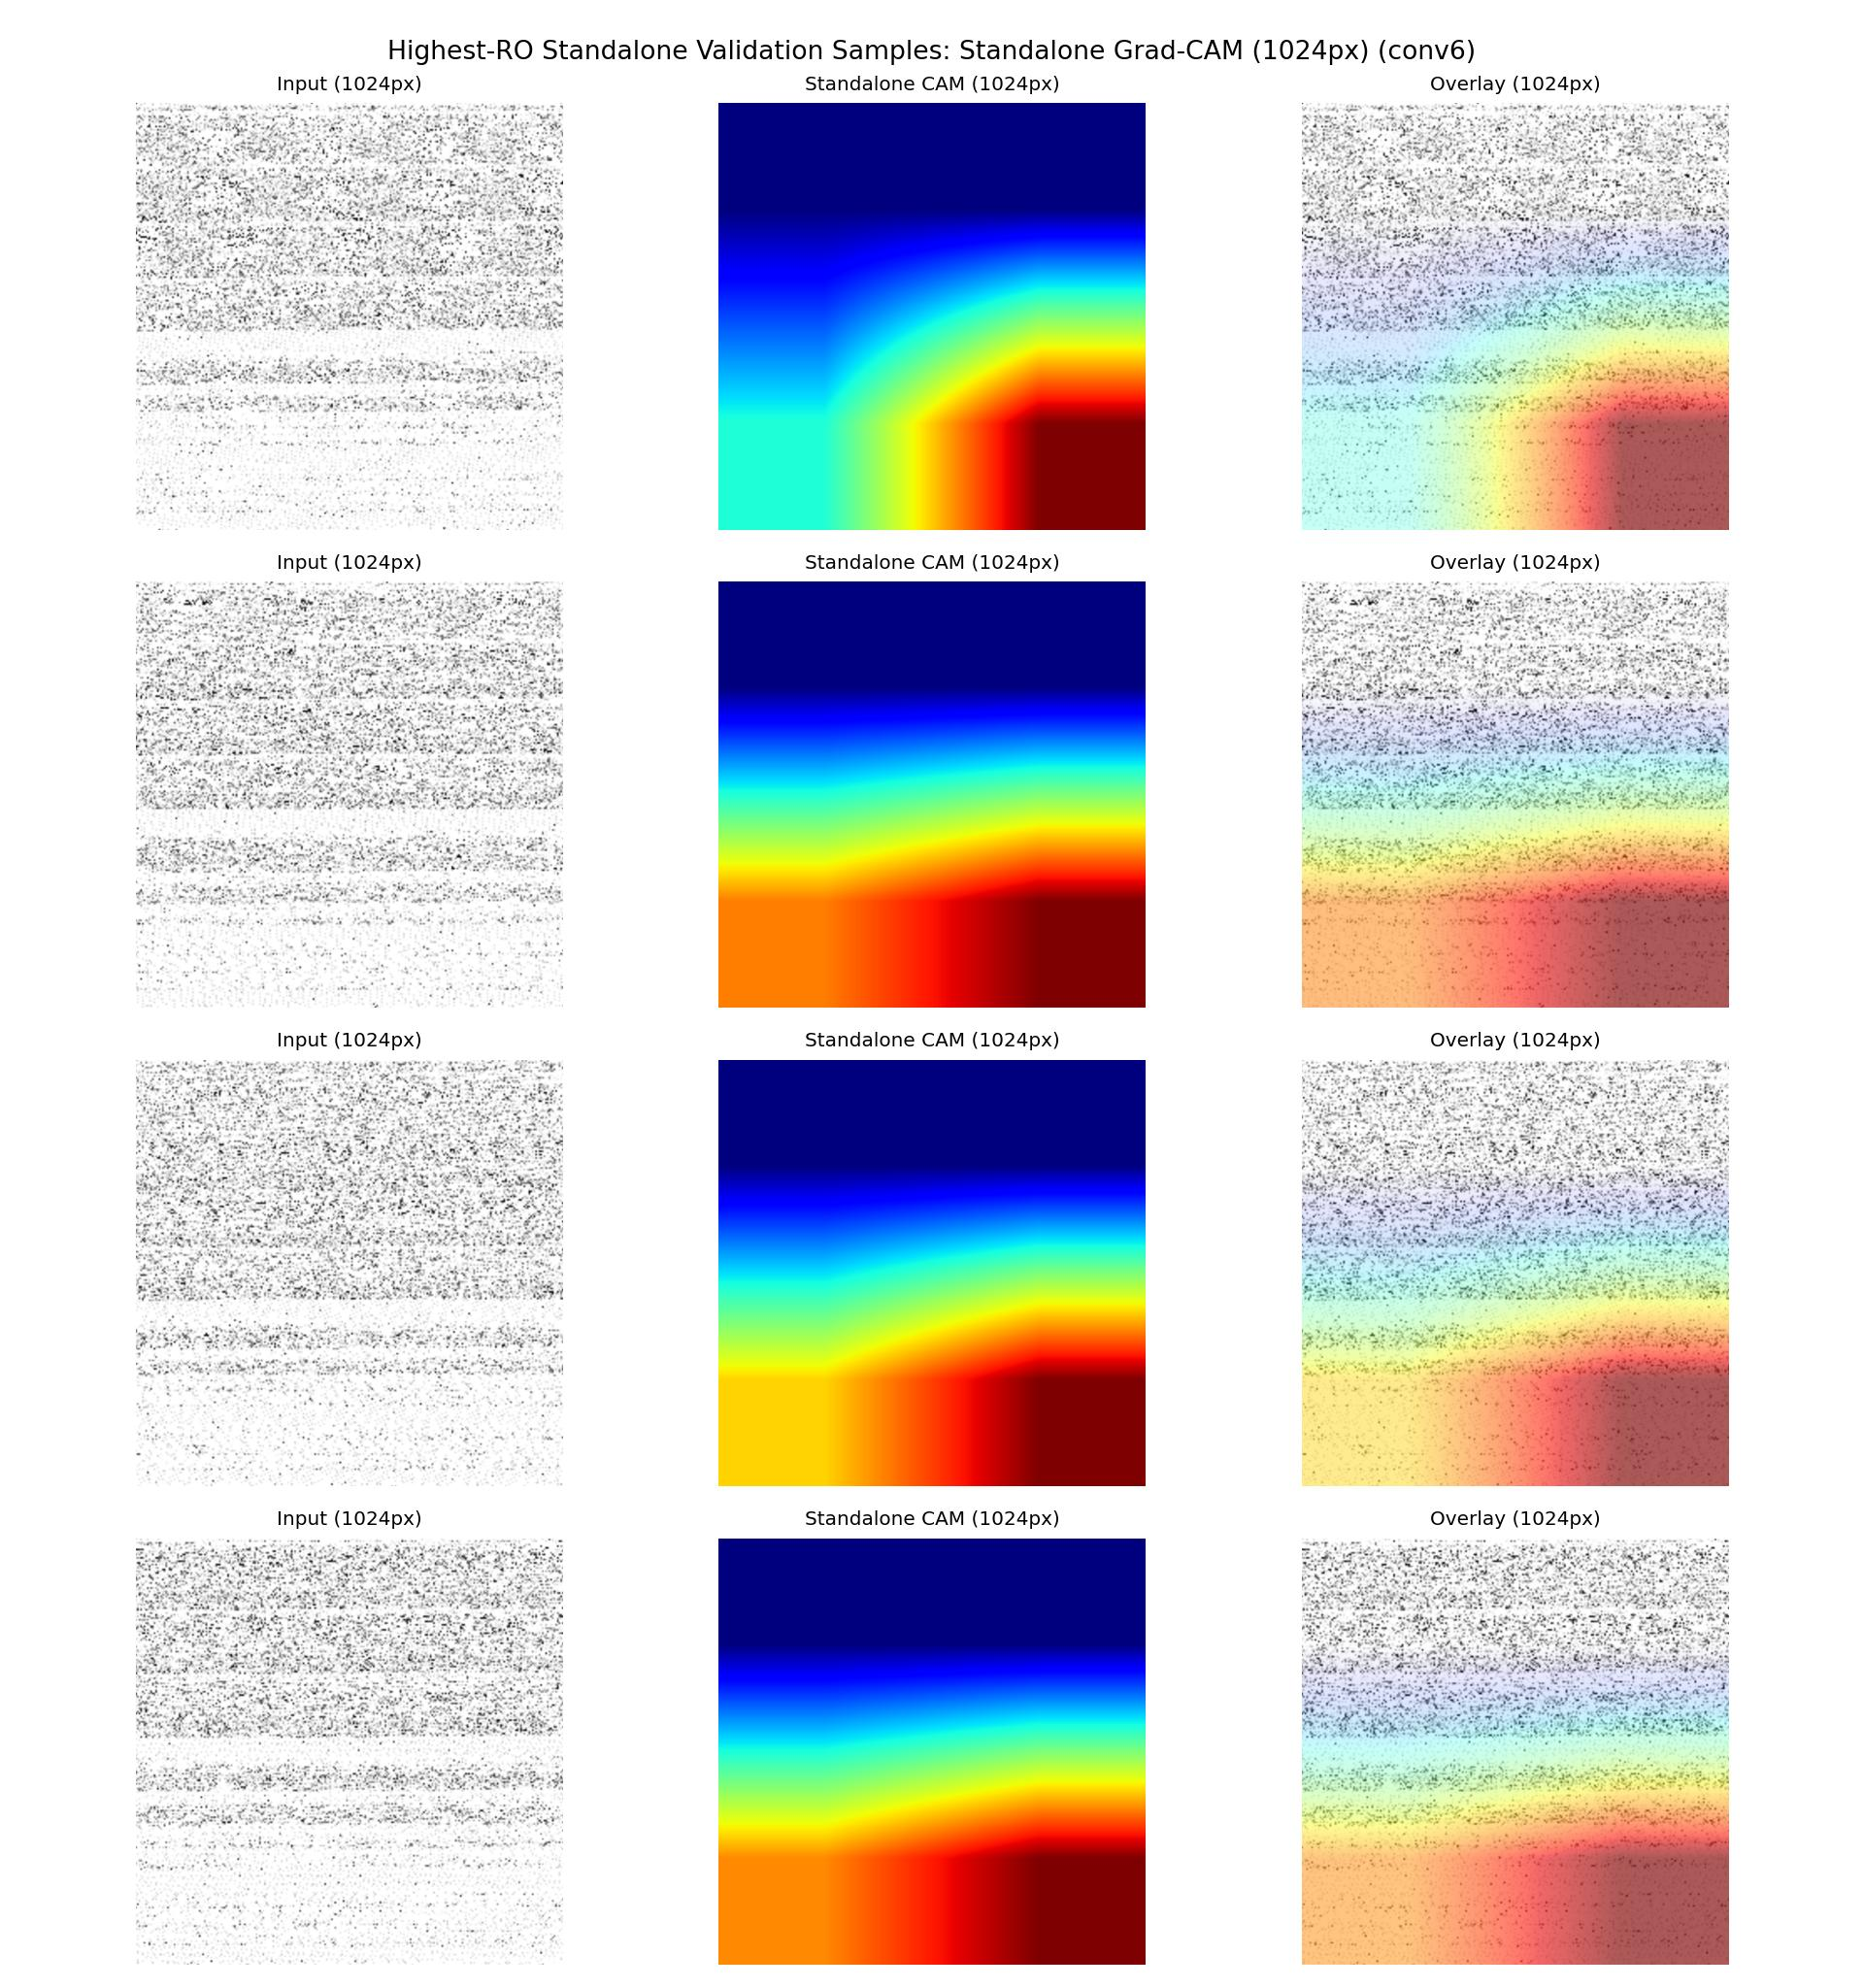
\includegraphics[width=0.82\linewidth]{figures/gradcam_example.pdf}
    \caption{Grad-CAM example for a malicious prediction. The highlighted regions show which parts of the bitstream image contribute most to the classifier output.}
    \label{fig:gradcam-example}
\end{figure}

The Grad-CAM examples show localized regions and bands with higher contribution. This supports the use of a spatial bitstream representation. It does not prove that the model identifies ring oscillators at the circuit level. It is only a qualitative check on the learned representation.

\section{Extended RO-Footprint Evaluation}
\label{sec:ro-footprint-evaluation}

The original dataset tests whether the classifier can separate benign Coyote bitstreams from RO-based malicious bitstreams. We also evaluate how detection changes as the RO footprint increases. This matters because high-density RO payloads are more relevant for power-stress and timing-fault scenarios.

Figure~\ref{fig:ro-footprint-detection} shows the extended RO-footprint result. Misses concentrate in the smallest RO-footprint bin. Detection becomes reliable for larger evaluated payloads. This suggests that the classifier is strongest for high-density RO attacks, while low-footprint payloads remain the harder case.

\begin{figure}[t]
    \centering
    % Replace with the exported RO-footprint plot from the presentation.
    % Recommended file name: figures/ro_footprint_detection.pdf
    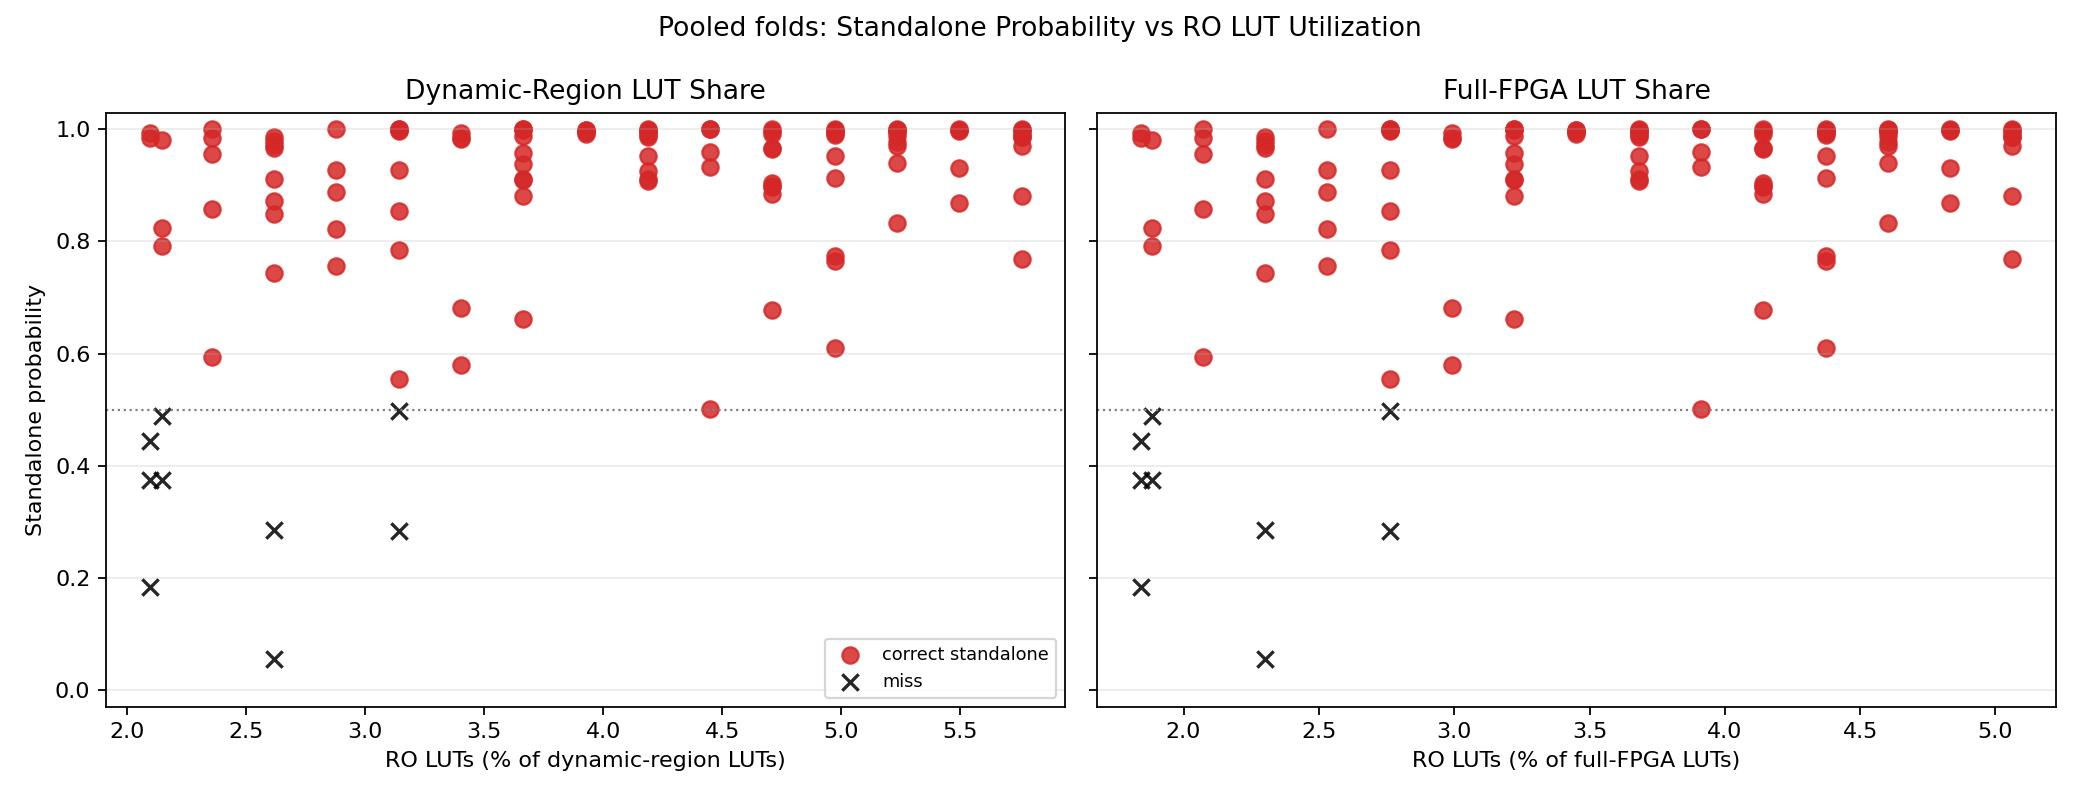
\includegraphics[width=0.82\linewidth]{figures/ro_footprint_detection.pdf}
    \caption{Detection across RO-footprint bins. Smaller RO payloads are harder to detect, while larger evaluated payloads are detected more reliably.}
    \label{fig:ro-footprint-detection}
\end{figure}

This result is important for interpreting the detector. The model does not provide complete coverage against all malicious circuits. It provides useful coverage for RO-based payloads, especially larger payloads that are more likely to create practical power-stress effects. The next chapter evaluates whether these CNN candidates can be synthesized into practical FPGA-resident checkers.